\documentclass[utf8]{beamer}
\usepackage{pgfpages}

\bibliographystyle{apalike}


\title{A genetic study of height in Human}
\subtitle{Application to the IMAGEN cohort}
\date{\today}
\author[Vincent Frouin]{Vincent Frouin, Yann LeGuenn}
\institute[CEA]{CEA - NeuroSpin}
%\titlegraphic{
\includegraphics[width=7cm]{graphics/your_image_here.png}}

\usetheme{cea}

\graphicspath{ {./images/} }
\usepackage{subfigure}

% uncomment if you do want notes
%\setbeameroption{show notes on second screen=right}

% comment if you do not want grey item
\setbeamercovered{transparent}
% comment if you do not want a summary at each section
\AtBeginSection[]{
    \begin{frame}{Summary}
        \small \tableofcontents[currentsection, hideothersubsections]
    \end{frame} 
}


\begin{document}

\begin{frame}
    \titlepage
\end{frame}

\begin{frame}
    \frametitle{Definitions}
    \framesubtitle{ }    
    \begin{block}{Phenotype (or trait)}
    Any observable characteristics of an individual  resulting from the interaction of the environment and \textbf{genotype}.
    \begin{itemize}
     \item Continuous, categorical
     \item Biochemical, physiological, anatomical
    \end{itemize}
    \end{block}
    
    \begin{block}{Genotype}
    The structural variants of the individual genome (with respect to an arbitrary reference)
    \begin{itemize}
    \item Variants may be SNPs (3M out of the 3.2B nucl. human genome) indel, repetitions
    \item Measured with DNA chips (1M, 750K sites), or sequencer (whole genome/exome ) 
    \item \textbf{Common} \textit{vs} rare variants
    \end{itemize}
    \end{block}
    
\end{frame}

%% ============================================================= %%
\section{Introduction on the height trait}

%% --------------------------------------------------------------- %
\begin{frame}
\frametitle{What do we know about human height and genetics ?}
\begin{itemize}
\item Human height is notoriously heritable phenotype . It is a classical example of a polygenic trait.
\begin{itemize}
\item Mendelian \textit{vs} Fisher architecture
\end{itemize}
\begin{center}
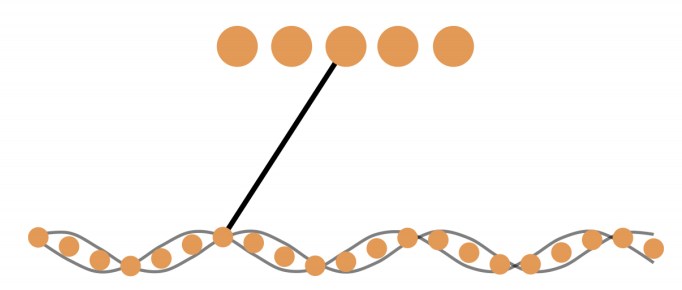
\includegraphics[height=1cm]{mono}
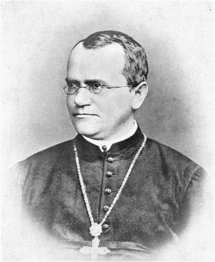
\includegraphics[height=1cm]{mendel}
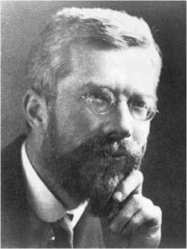
\includegraphics[height=1cm]{fisher}
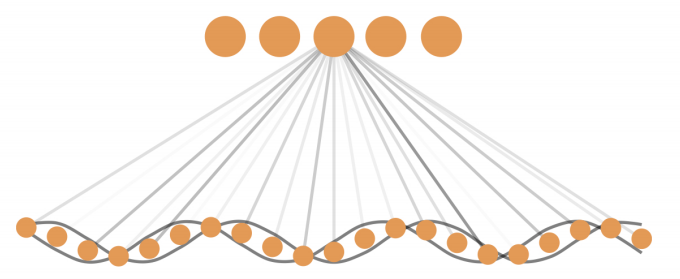
\includegraphics[height=1cm]{infinitesimal}\end{center}

\item A few figures:
\begin{itemize}
\item up to 80\% based on twin studies \cite{Yang2010}
\item 60-70\% from \cite{Yang2015}
\end{itemize}


\item The height heritability is manifesting differently depending of the kind of tools used to investigate this issue.
\end{itemize}
\end{frame}

%%% ============================================================= %%
\section{Material and methods}
%% --------------------------------------------------------------- %
\begin{frame}
\frametitle{The height trait in Human}


The variance explained by the geneticsin the variance of height depends on whether or not  causal
variant localisation is searched.
	\begin{block}{No causal variant localisation}
	\begin{itemize}
	\item \textbf{Reference}: heritability $h^2$ (narrow sense)  with twin studies
	\item for height: 65 \% of variance found \cite{}
	\end{itemize}
	\end{block}
	
	\begin{block}{With causal variant localisation}
	\begin{itemize}
	\item \textbf{Reference}: huge genome wide analysis or meta analysis
	\item for height: 16 \% meta w/ $180,000$ subjects \cite{LangoAllen2010}
	\end{itemize}
	\end{block}

\end{frame}

%% --------------------------------------------------------------- %
\begin{frame}
\frametitle{Assessing the association height-genotype (1)}
Several way to assess empirically the part of genetic variance in the 
phenotypic variance:
\begin{itemize}
\item A fraction of $h^2$ may be found with/out variant localization:
	\vspace{.5cm}
	\begin{enumerate}
	\item Variance explained by whole genome (GCTA, MEGHA)
	\item Univariate association analysis (GWAS)
	\item Multivariate association analysis
	\item Polygenic scores: association analysis with a signature built 
	from a set of SNPs obtained elsewhere (eg. meta-analysis)
	\end{enumerate}
	
\vspace{.5cm}
\item Depending on the method used, causal variants will be obtained
\end{itemize}
\end{frame}


%% --------------------------------------------------------------- %
\begin{frame}
\frametitle{Assessing the association height-genotype (2)}
Recently \cite{Zhang2011} studied an Adriatic island population to
replicate findings in "height and genetics" and to reveal potential 
island specificities of the population.

\vspace{1cm}
\textbf{Questions}:
\begin{itemize}
\item Replicate the reference figures on the IMAGEN data,
\item Identify specific aspects of the IMAGEN cohort.
\end{itemize}

\end{frame}

%% --------------------------------------------------------------- %
\begin{frame}
\frametitle{Assessing the association height-genotype (3)}
\framesubtitle{The data}
Ground Truth:
\begin{itemize}
	\item Method without local information on variants:
	\begin{itemize}
	\item $h^2$ should be ~65\%
	\end{itemize}
	\item Method with local information on variants:
	\begin{itemize}
	\item 180 pairs (SNP, univariate weight) \cite{LangoAllen2010}.
	\item 180 SNPs explains $10 to 16\%$
	\end{itemize}
\end{itemize}

\vspace{0.5cm}
IMAGEN:
\begin{itemize}
\item Genotyping data: $1,835$ subjects and $477,245$ SNPs
\item Complete data set (covariate variables, height, genetics): 
$1,701$ subjects $215,378$ informative SNPs 
\end{itemize}
\end{frame}



%% ============================================================= %%
\section{Results}


%% --------------------------------------------------------------- %
\begin{frame}
\frametitle{Genetics specificities of IMAGEN population }
\begin{itemize}
\item 173 out of the 180 SNPs were available from the imputed IMAGEN data
\end{itemize}
\tiny
\begin{tabular}{|c|c|c|c|}
\hline     &  Maf-1000genome   &    Maf-IMAGEN   &   Diff \\
\hline \hline  rs11205277 & 0.42&  0.442475 & 0.022475\\
\hline  rs10863936 & 0.47 & 0.476827 & 0.006827\\
\hline  rs4601530  & 0.26 & 0.254907 & 0.005093\\
\hline  rs6699417  & 0.39 & 0.410033 &  0.020033\\
\hline  rs1738475 &  0.41 & 0.390403 & 0.019597\\
\hline
\end{tabular} 
\end{frame}

%% --------------------------------------------------------------- %
\begin{frame}
\frametitle{Genetics specificities of IMAGEN population }

Statistics summary on the MAF difference:
\tiny
\begin{itemize}
\item Max:  0.393478735005
\item Min:  3.27153762268e-05
\item Mean:  0.0159850227873
\item Quantile 75\% (0.015802) and 95\% (0.038332)
\end{itemize}

\vspace{0.5cm}
\normalsize
Snps with difference in MAF in the 95\% quantile:\\
\vspace{0.5cm}
\tiny
\begin{tabular}{|c|c|c|c|c|c|c|}
\hline     &  A1 &  A2 &  Maf-1000genome &   Beta     & Maf-IMAGEN   &   Diff \\
\hline
\hline rs2284746 & G & C & 0.48 &-0.040 & 0.521810 & 0.041810 \\
\hline rs6470764 & C & T & 0.20 &-0.050  &  0.478462 & 0.278462 \\
\hline rs1257763 & G & A & 0.04 & 0.069  &  0.433479 & 0.393479 \\
\hline rs8181166 & C & G & 0.47 &-0.026  &  0.508724 & 0.038724 \\
\hline rs1814175 & C & T & 0.34 & 0.022  &  0.415758 & 0.075758 \\
\hline rs5742915 & C & T & 0.54 &-0.031  &  0.456379 & 0.083621 \\
\hline rs7178424 & C & T & 0.47 &-0.021  &  0.430207 & 0.039793 \\
\hline rs26868   & A & T & 0.54 &-0.034    &  0.460742 &  0.079258 \\
\hline rs2665838 & C & G & 0.27 & 0.042  &  0.231189 & 0.038811 \\
\hline
\end{tabular} 
\end{frame}

%% --------------------------------------------------------------- %
\begin{frame}
\frametitle{Univariate approach}
Covariate: Age, ScanningCentre, Sex. $\#$Subjects: 1596.
\vspace{1cm}
\begin{itemize}
\item Univariate results:
	\begin{itemize}
	\item numbers of significant p values *un*corrected 23 over 173
	\item numbers of significant corrected p values corrected 2 over  173
	\item $[$rs2778031 rs11259936$]$, pval =  [ 0.04886258  0.04886258],  correlation =  [ 0.0862132  -0.08950396]
	\item SNPs in the 173 of interest?
	\end{itemize}
\vspace{0.5cm}
\item Variance explained by the 2 significant SNPs is $1.5\%$ of the height var
      ($R^2$ of the linear model - scipy lm.score())
\end{itemize}

\end{frame}

%% --------------------------------------------------------------- %
\begin{frame}
\frametitle{Multivariate approach}
\end{frame}



%% --------------------------------------------------------------- %
\begin{frame}
\frametitle{Polygenic score approach}
\end{frame}

%% --------------------------------------------------------------- %
\begin{frame}
\frametitle{By the way, the hippocampus size}
\end{frame}


%% ============================================================= %%
\begin{frame}[shrink=50,t]
\frametitle{References}
\small\bibliography{height}
\end{frame}

%\begin{frame}[t,allowframebreaks]
%\frametitle{References}
%\bibliography{height}
%\end{frame}


\end{document}
